\documentclass[aspectratio=169,14pt]{beamer}
\usepackage[utf8]{inputenc}
\usepackage[T1]{fontenc}
\usetheme{Madrid}
\setbeamertemplate{navigation symbols}{}
\title{The AI Lemons Problem}
\subtitle{How AI adoption can unravel prediction markets}
\begin{document}
\begin{frame}[plain]
\titlepage
\end{frame}

\begin{frame}{AI can improve prediction while undermining market viability}
\textbf{Higher AI penetration widens spreads and drives out uninformed traders.}
\begin{itemize}
  \item The informed share of order flow rises with AI adoption
  \item Uninformed participation is endogenous to the spread
\end{itemize}
\begin{block}{Takeaway}The market can collapse even as conditional prediction improves.\end{block}
\end{frame}

\begin{frame}{Prediction markets need counterparties, not information alone}
\textbf{The paper makes participation, rather than price accuracy alone, the central margin.}
\begin{itemize}
  \item Liquidity traders and recreational users sustain two-sided order flow
  \item Their willingness to trade falls when spreads become costly
\end{itemize}
\begin{block}{Takeaway}Market composition determines whether information aggregation remains possible.\end{block}
\end{frame}

\begin{frame}{AI adoption creates a self-reinforcing adverse-selection spiral}
\begin{figure}\centering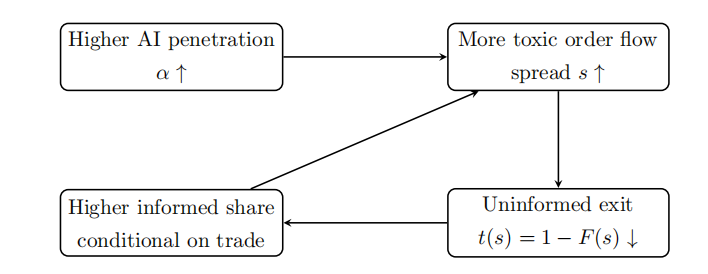
\includegraphics[width=0.86\textwidth]{../beamer-progress-draft/assets/ai-adverse-selection-spiral.png}
\caption{AI adoption raises informational asymmetry, spreads, and uninformed exit.}
\end{figure}
\textit{Participation feedback turns asymmetry into possible collapse.}
\end{frame}

\begin{frame}{The model combines informed trading with endogenous participation}
\begin{itemize}
  \item Binary prediction contract with state V in \{0,1\}
  \item AI-informed traders have superior predictive ability
  \item Uninformed traders have heterogeneous participation values z
  \item Competitive market makers price orders conditional on direction
\end{itemize}
\end{frame}

\begin{frame}{Pricing and participation form a fixed-point problem}
\begin{equation*}s = \frac{\alpha}{2[\alpha + (1-\alpha)(1-F(s))]}\end{equation*}
\begin{itemize}
  \item s: equilibrium half-spread
  \item alpha: AI penetration
  \item F(s): share of uninformed traders priced out
\end{itemize}
\textit{A wider spread reduces participation and makes order flow more informative.}
\end{frame}

\begin{frame}{More AI makes every order more revealing to the market maker}
\textbf{The gap between buy probabilities across states equals the AI penetration rate alpha.}
\begin{itemize}
  \item AI traders buy when V = 1 and sell when V = 0
  \item Uninformed traders trade only when z exceeds the spread
\end{itemize}
\begin{block}{Takeaway}Higher alpha raises adverse-selection pricing pressure directly.\end{block}
\end{frame}

\begin{frame}{Higher AI penetration shifts the spread schedule toward collapse}
\begin{figure}\centering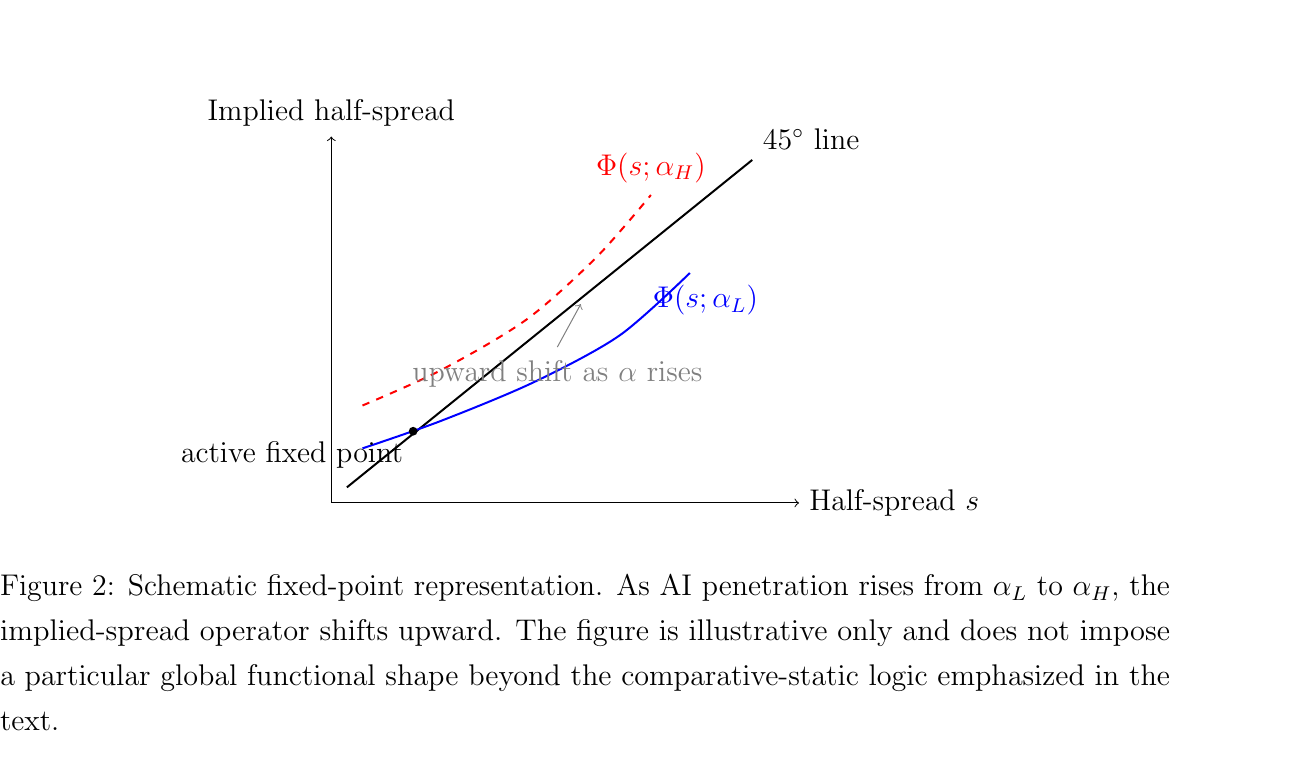
\includegraphics[width=0.86\textwidth]{../beamer-progress-draft/assets/fixed-point-schematic.png}
\caption{Schematic fixed-point representation from the paper.}
\end{figure}
\end{frame}

\begin{frame}{AI penetration above the threshold eliminates active equilibrium}
\begin{block}{Result}If alpha > 2 z-bar, no active equilibrium exists and the collapsed equilibrium is unique.\end{block}
\textit{Intuition:} The minimum AI-induced spread exceeds the strongest non-informational participation value.
\end{frame}

\begin{frame}{The gradual phase is wider spreads and fewer ordinary participants}
\textbf{Before collapse, equilibrium spreads rise and participation falls with AI penetration.}
\begin{itemize}
  \item The spread operator is increasing in s and alpha
  \item Participation is t(alpha) = 1 - F(s(alpha))
\end{itemize}
\begin{block}{Takeaway}The collapse theorem is the endpoint of a continuous deterioration mechanism.\end{block}
\end{frame}

\begin{frame}{AI rents are transfers, while participation creates baseline surplus}
\textbf{In the baseline welfare criterion, AI does not create direct productive surplus.}
\begin{itemize}
  \item AI rents equal spread losses borne by uninformed traders
  \item Market makers earn zero expected profit
  \item Real surplus comes from non-informational participation values
\end{itemize}
\begin{block}{Takeaway}Private profitability and social value need not move together.\end{block}
\end{frame}

\begin{frame}{Participation-based welfare declines with AI penetration}
\begin{equation*}W(\alpha) = (1-\alpha) \int_{s^*(\alpha)}^{\bar z} z \,dF(z)\end{equation*}
\begin{itemize}
  \item W(alpha): baseline social welfare
  \item s*(alpha): selected active-equilibrium spread
  \item The integral captures surviving participation value
\end{itemize}
\textit{AI reduces welfare by shrinking the set of traders who remain active.}
\end{frame}

\begin{frame}{Private AI adoption can exceed the planner's optimum}
\begin{block}{Result}With non-negative adoption costs and the baseline welfare criterion, the planner chooses the lowest feasible adoption level.\end{block}
\textit{Intuition:} Adopters capture private rents but do not internalize the participation externality imposed on other traders.
\end{frame}

\begin{frame}{Market design can target participation rather than price accuracy}
\begin{itemize}
  \item Participation subsidies reduce the effective cost of trading
  \item AI adoption taxes reduce privately chosen adoption
  \item Public information can reduce the AI informational edge
  \item AMM liquidity support addresses the analogous withdrawal spiral
\end{itemize}
\end{frame}

\begin{frame}{Extensions preserve the participation feedback}
\begin{itemize}
  \item Imperfect AI replaces alpha with effective informed intensity
  \item Heterogeneous quality preserves the adverse-selection feedback
  \item Dynamic persistence creates path dependence and hysteresis
  \item AMMs and multi-market settings retain the core participation force
\end{itemize}
\end{frame}

\begin{frame}{The theory yields testable predictions but not current-market evidence}
\textbf{The paper identifies empirical implications rather than claiming that prediction markets have already collapsed.}
\begin{itemize}
  \item AI exposure should predict wider spreads
  \item Wider spreads should reduce less-informed participation
  \item Order flow should become more concentrated in informed traders
\end{itemize}
\begin{block}{Takeaway}Whether real markets are near the threshold remains an open empirical question.\end{block}
\end{frame}

\begin{frame}{AI creates an efficiency-survival trade-off}
\vfill
\begin{block}{Takeaway}AI may improve price discovery while destroying the participation base that makes price discovery possible.\end{block}
\vfill
\end{frame}
\end{document}
